%\documentclass[
  bibliography=totoc,     % Literatur im Inhaltsverzeichnis
  captions=tableheading,  % Tabellenüberschriften
  titlepage=firstiscover, % Titelseite ist Deckblatt
]{scrartcl}

% Paket float verbessern
\usepackage{scrhack}

% Warnung, falls nochmal kompiliert werden muss
\usepackage[aux]{rerunfilecheck}

% unverzichtbare Mathe-Befehle
\usepackage{amsmath}
% viele Mathe-Symbole
\usepackage{amssymb}
% Erweiterungen für amsmath
\usepackage{mathtools}

% Fonteinstellungen
\usepackage{fontspec}
% Latin Modern Fonts werden automatisch geladen
% Alternativ zum Beispiel:
%\setromanfont{Libertinus Serif}
%\setsansfont{Libertinus Sans}
%\setmonofont{Libertinus Mono}

% Wenn man andere Schriftarten gesetzt hat,
% sollte man das Seiten-Layout neu berechnen lassen
\recalctypearea{}

% deutsche Spracheinstellungen
\usepackage[ngerman]{babel}


\usepackage[
  math-style=ISO,    % ┐
  bold-style=ISO,    % │
  sans-style=italic, % │ ISO-Standard folgen
  nabla=upright,     % │
  partial=upright,   % │
  mathrm=sym,        % ┘
  warnings-off={           % ┐
    mathtools-colon,       % │ unnötige Warnungen ausschalten
    mathtools-overbracket, % │
  },                       % ┘
]{unicode-math}

% traditionelle Fonts für Mathematik
\setmathfont{Latin Modern Math}
% Alternativ zum Beispiel:
%\setmathfont{Libertinus Math}

\setmathfont{XITS Math}[range={scr, bfscr}]
\setmathfont{XITS Math}[range={cal, bfcal}, StylisticSet=1]

% Zahlen und Einheiten
\usepackage[
  locale=DE,                   % deutsche Einstellungen
  separate-uncertainty=true,   % immer Unsicherheit mit \pm
  per-mode=symbol-or-fraction, % / in inline math, fraction in display math
]{siunitx}

% chemische Formeln
\usepackage[
  version=4,
  math-greek=default, % ┐ mit unicode-math zusammenarbeiten
  text-greek=default, % ┘
]{mhchem}

% richtige Anführungszeichen
\usepackage[autostyle]{csquotes}

% schöne Brüche im Text
\usepackage{xfrac}

% Standardplatzierung für Floats einstellen
\usepackage{float}
\floatplacement{figure}{htbp}
\floatplacement{table}{htbp}

% Floats innerhalb einer Section halten
\usepackage[
  section, % Floats innerhalb der Section halten
  below,   % unterhalb der Section aber auf der selben Seite ist ok
]{placeins}

% Seite drehen für breite Tabellen: landscape Umgebung
\usepackage{pdflscape}

% Captions schöner machen.
\usepackage[
  labelfont=bf,        % Tabelle x: Abbildung y: ist jetzt fett
  font=small,          % Schrift etwas kleiner als Dokument
  width=0.9\textwidth, % maximale Breite einer Caption schmaler
]{caption}
% subfigure, subtable, subref
\usepackage{subcaption}

% Grafiken können eingebunden werden
\usepackage{graphicx}

% schöne Tabellen
\usepackage{tabularray}
\UseTblrLibrary{booktabs, siunitx}

% Verbesserungen am Schriftbild
\usepackage{microtype}

% Literaturverzeichnis
\usepackage[
  backend=biber,
]{biblatex}
% Quellendatenbank
\addbibresource{lit.bib}
\addbibresource{programme.bib}

% Hyperlinks im Dokument
\usepackage[
  german,
  unicode,        % Unicode in PDF-Attributen erlauben
  pdfusetitle,    % Titel, Autoren und Datum als PDF-Attribute
  pdfcreator={},  % ┐ PDF-Attribute säubern
  pdfproducer={}, % ┘
]{hyperref}
% erweiterte Bookmarks im PDF
\usepackage{bookmark}

% Trennung von Wörtern mit Strichen
\usepackage[shortcuts]{extdash}

\author{%
  Vincent Wirsdörfer\\%
  \href{mailto:vincent.wirsdoerfer@udo.edu}{authorA@udo.edu}%
  \and%
  Joris Daus\\%
  \href{mailto:joris.daus@udo.edu}{authorB@udo.edu}%
}
\publishers{TU Dortmund – Fakultät Physik}


%\begin{document}
\section{Zielsetzung}


Das konkrete Ziel des folgend protokollierten Versuchs besteht darin den Elastizitätsmodul von Metallen verschiedener
Legierungen zu bestimmen. Ferner werden die empirisch ermittelten Werte mit der Literatur verglichen und somit deren
Aussagekraft bewertet.

\section{Theorie}
\label{sec:Theorie}
An einem Körper lässt sich genau dann eine Veränderung der Gestalt und des Volumens feststellen, wenn eine Kraft auf die
Oberfläche des Körpers einwirkt. Oftmals bezieht man diese Krafteinwirkung auf Flächeneinheiten, weswegen die physikalisch 
erhaltende Größe in diesem Fall die Spannung ist. Dabei muss jedoch zwischen zwei Spannungskomponenten unterschieden werden.
Einerseits gibt es den senkrecht zur Oberfläche stehenden Anteil der Spannung, welcher als \emph{Normalenspannung} $\sigma$
bezeichnet wird. Andererseit existiert zudem ein parallel zur Oberfläche stehender Anteil der Spannung. Dieser Anteil
heißt \emph{Tangentialspannung}. Ist nun die relative Änderung $\sfrac{\increment L}{L}$ einer linearen Körperdimension
hinreichend klein, so lässt sich ein proportionaler Zusammenhang zwischen dieser Änderung und der angreifenden Normalenspannung
$\sigma$ konstatieren. Präziser ausgedrückt wird dieser Zusammenhang durch das \emph{Hook'sche Gesetz}:

\begin{equation}
    \sigma = E\frac{\increment L}{L}
    \label{eqn:Hook}
\end{equation}

\noindent Hierbei wird der Proportionalitätsfaktor dieser Gleichung als \emph{Elastizitätsmodul} beschrieben. Dieser 
repräsentiert eine wichtige Materialkonstante in der Werkstofftechnik.\\
\noindent Anhand von Gleichung \eqref{eqn:Hook} lässt sich nun vermuten, dass der Elastizitätsmodul durch eine bestimmte Messvorrichtung
und triviales Umstellen der Gleichung einfach zu errechnen ist. Aufgrund der Tatsache, dass solch eine Vorrichtung nicht immer
gewährleistet werden kann, wird sich bei diesem Versuch einer anderen Methodik, nämlich der Biegung von elastischen
Stäben, bedient. Die theoretischen Grundgedanken hinter diesem Ansatz werden im Folgenden näher erläutert.

\subsection{Berechnung des E-Moduls bei einseitiger Einspannung des Stabes}
\label{sec:Einseitig_t}

Wie bereits in der Theorie angeklungen, bedingt die Dehnung des Stabes nach Gleichung \eqref{eqn:Hook} eine Biegung des Körpers
was letztlich in einer Deformation resultiert. Dementsprechend muss eine Versuchsapperatur gefunden werden, welche es erlaubt,
die Durchbiegung $D(x)$ an verschiedenen Stellen $x$ zu messen. Eine solche Apperatur wird in Abbildung \ref{fig:Durchbiegung}
dargestellt.

\begin{figure}[H]
    \centering
    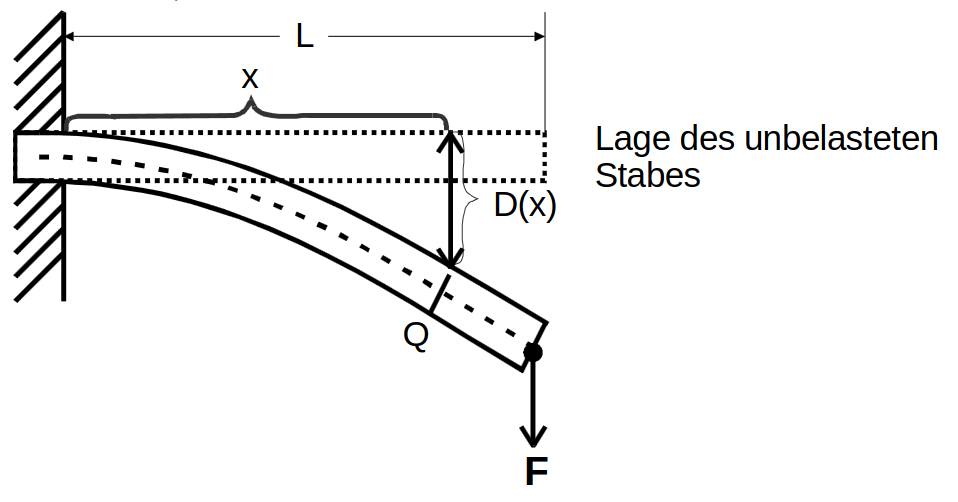
\includegraphics[height=5cm]{./content/Durchbiegung.png}
    \caption{Durchbiegung eines elastischen Stabes bei einseitiger Aufhängung}
    \label{fig:Durchbiegung}
\end{figure}

\noindent Es soll somit eine Menge von Wertepaaren $\{D(x),x\}$ bestimmt werden. Diese Messreihe wird dazu verwendet, den E-Modul
des Stabes zu berechnen, da die Funktion $D(x)$ abhängig von $E$ ist. Die Gleichung muss somit nach $E$ umgestellt werden, um 
einen Wert für den Elastizitätsmodul zu erhalten. Doch wie konkretisiert sich die Funktion $D(x)$ mathematisch genau?\\
An der Abbildung \ref{fig:Durchbiegung} ist zu erkennen, dass Kräftepaare auf den Stab einwirken, weswegen eine
\emph{Drehmomentgleichung} aufgestellt werden muss, um einen Ausdruck für $D(x)$ zu finden. Ferner zeigt die Abbildung, dass die Kraft $F$
auf den Querschnitt $Q$ ein Drehmoment $M_F$ bewirkt, welcher den Querschnitt aus seiner Ausgangslage verdreht. Dadurch werden,
die oberen Schichten des Stabes gedehnt und die unteren Schichten gestaucht. Elastische Eigenschaften des Stabes erzeugen jedoch
innere Normalenspannungen, welche dieser Biegung entgegenwirken. Zwischen der oberen und unteren Schicht existiert eine Fläche,
wo sich die Zugspannungen und die Druckspannungen genau ausgleichen, weswegen hier in Summe keine Spannungen 
auftreten. Daher wird diese Fläche auch als \emph{neutrale Faser}\footnote{In Abb. \ref{fig:Durchbiegung} wird ihre Schnittline als gestrichelte Linie dargestellt.} bezeichnet.
Die entgegenwirkenden jedoch betragsmäßig äquivalenten Zug- und Druckspannungen erzeugen ein Drehmoment $M_\sigma$, welches sich wie folgt
berechnet lässt:

\begin{equation}
\label{eqn:Moments}
    M_\sigma = \int_Q y\sigma(y)\symup{d}q 
\end{equation}

\noindent Hierbei bezeichnet $y$ den Abstand des Flächenelements d$q$ zur neutralen Faser.\\
Wenn nun, wie in Abbildung \ref{fig:Durchbiegung} gezeigt, eine Kraft $F$, mit dem Hebelarm $L-x$ an einem Punkt des Stabes angreift, bedeutet dies
ein weiteres Drehmoment $M_F$ mit
\begin{equation}
\label{eqn:MomentF}
    M_F = F\left(L-x\right).
\end{equation}

\noindent Die Deformation stellt sich nun so sein, dass ein Gleichgewicht der Momente \eqref{eqn:Moments} und \eqref{eqn:MomentF} herrscht:

\begin{equation}
\label{eqn:Moment1}
    \int_Q y\sigma(y)\symup{d}q =F\left(L-x\right)
\end{equation}

\noindent Nun wird jedoch versucht, einen Ausdruck für die Normalenspannung $\sigma(y)$ zu finden. Dies kann am besten mittels
einer dazu passenden Abbildung illustriert werden:

\begin{figure}
    \centering
    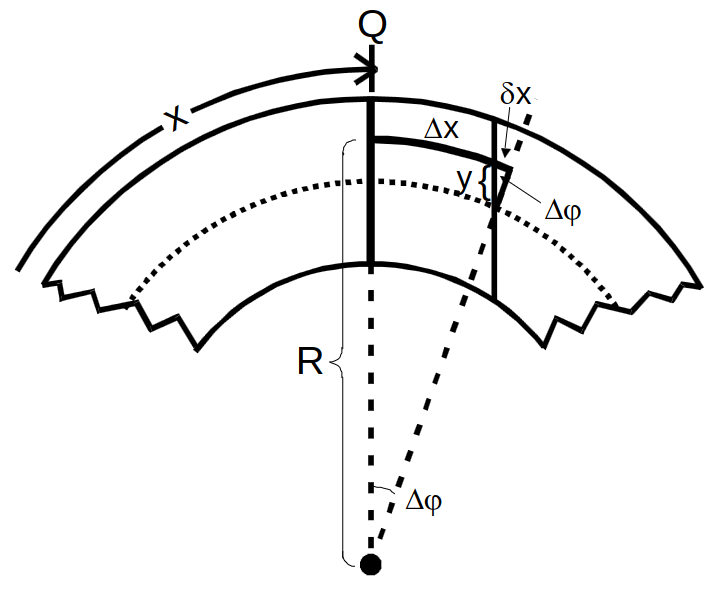
\includegraphics[height=7cm]{./content/Trigonometrie.png}
    \caption{Skizze zur Normalenspannung $\sigma(y)$}
    \label{fig:Trigonometrie}
\end{figure}

\noindent Mit Hilfe von Abbildung \ref{fig:Trigonometrie} lassen sich nun trigonometrische Beziehungen einfacher erkennen, weswegen
wir $\sigma(y)$ über den Ausdruck

\begin{equation}
\label{eqn:Normalenspannung}
    \sigma(y) = E\frac{\delta x}{\Delta x}
\end{equation}

\noindent umschreiben können. Dabei steht $\delta x$ für eine kleine Längenänderung der Faser mit Ursprungslänge $\Delta x$. Es gilt:
$\delta x << \Delta x$. Aus der Abbildung \ref{fig:Trigonometrie} resultiert zudem 

\begin{equation*}
    \delta x = y\Delta\varphi = y\frac{\Delta x}{R},
\end{equation*}

\noindent wobei $R$ nach der Abbildung für den Krümmungsradius der Faser an der Stelle x steht. Unter Verwendung folgender Beziehung aus der 
Differentialgeometrie

\begin{equation*}
    \frac{1}{R} \approx \frac{\symup{d}²D}{\symup{d}x²}
\end{equation*}

\noindent unter der Voraussetzung, dass $R$ hinreichend groß ist und $\sfrac{\symup{d}²}{\symup{d}x²}$ gilt. Somit lässt sich
Gleichung \eqref{eqn:Normalenspannung} umschreiben zu

\begin{equation*}
    \sigma(y) = Ey\frac{\symup{d}²D}{\symup{d}x²}
\end{equation*}

\noindent Durch Einsetzen in Gleichung \eqref{eqn:Moment1} lässt sich der Ausdruck

\begin{equation}
\label{eqn:Moment2}
    E\frac{\symup{d}²D}{\symup{d}x²}\int_Q y²\symup{d}q = F\left(L-x\right)
\end{equation}

\noindent mit

\begin{equation*}
    I \coloneqq \int_Q y²\symup{d}q(y)
\end{equation*}

\noindent als \emph{Flächenträgheitsmoment} definieren. Unter Berücksichtigung der Tatsache, dass $D(0) = \sfrac{\symup{d}D}{\symup{d}x} = 0$ gilt, ergibt die zweifache Integration
von \eqref{eqn:Moment2} letztlich den Ausdruck

\begin{equation}
    D(x) = \frac{F}{2EI}\left(Lx²-\frac{x³}{3}\right)
    \label{eqn:Biegung_einseitig}
\end{equation}

\subsection{Berechnung des E-Moduls bei zweiseitiger Einspannung des Stabes}

Eine weitere Möglichkeit den E-Modul eines Stabes zu bestimmen ist die zweiseitige Einspannung des Körpers. Hierbei werden
analoge mathematische Ansätze wie im vorherigen Kapitel \autoref{sec:Einseitig_t} verwendet. Im Vergleich dazu ändert sich jedoch 
die Versuchsapperatur, was in der folgenden Abbildung wiedergegeben wird.

\begin{figure}
    \centering
    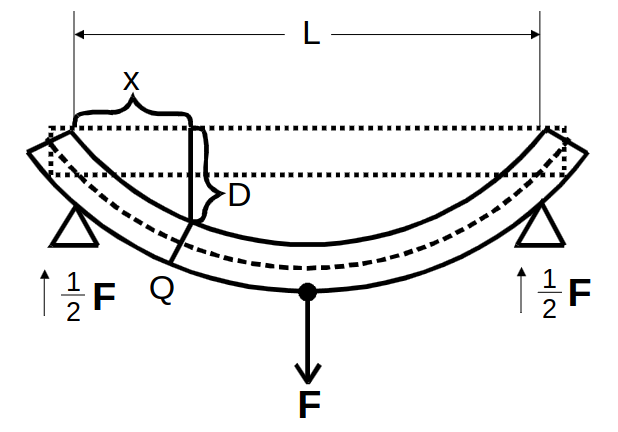
\includegraphics[height=7cm]{./content/Zweiseitig.png}
    \caption{Durchbiegung eines elastischen Stabes bei zweiseitiger Aufhängung}
    \label{fig:Zweiseitig}
\end{figure}

\noindent In der Abbildung \ref{fig:Zweiseitig} ist zu sehen, dass der Stab nun an zwei Seiten eingespannt ist und eine Krafteinwirkung $F$
in der Stabmitte erfährt. Somit greift nun die Kraft $\sfrac{F}{2}$ an den jeweiligen Enden des Stabes an, weswegen effektiv
zwei Drehmomentgleichungen für die Enden des Stabes entstehen, welche im Folgenden schrittweise hergeleitet werden.\\
\noindent Für das linke Ende des Stabes ergibt sich mit einer Kraft von $-\sfrac{F}{2}$ und einem Hebelarm $x$ ein Drehmoment $M_{F_1}$ von

\begin{align*}
    M_{F_1} &= -\frac{F}{2}\cdot x & &\text{für}\,\, 0 \leq x \leq \frac{L}{2}.
\end{align*}

\noindent Trivialerweise ergibt sich dann ein Drehmoment $M_{F_2}$ mit

\begin{align*}
    M_{F_2} &= -\frac{F}{2}\left(L-x\right) & &\text{für}\,\, \frac{L}{2} \leq x \leq L 
\end{align*}

\noindent In Anbetracht von Gleichung \eqref{eqn:Moment2} bedeutet dies spezifisch:

\begin{align*}
    \frac{\symup{d}²D}{\symup{d}x²} &= -\frac{F}{2EI}x & &\text{für}\,\, 0 \leq x \leq \frac{L}{2}\\
    \frac{\symup{d}²D}{\symup{d}x²} &= -\frac{F}{2EI}\left(L-x\right) & &\text{für}\,\, \frac{L}{2} \leq x \leq L
\end{align*}

\noindent Die Integration beider Gleichungen nach $x$ liefert folgende Ausdrücke:

\begin{align*}
    \frac{\symup{d}D}{\symup{d}x} &= -\frac{F}{4EI}x²+C_1 & &\text{für}\,\, 0 \leq x \leq \frac{L}{2}\\
    \frac{\symup{d}D}{\symup{d}x} &= -\frac{F}{2EI}\left(Lx-\frac{x²}{2}\right)+C_2 & &\text{für}\,\, \frac{L}{2} \leq x \leq L
\end{align*}

\noindent Im Vergleich zur einseitigen Methode können hier die Integrationskonstanten $C_1$ und $C_2$ nicht Null gesetzt werden,
in der Stabmitte eine horizontale Tangente an der Biegkurve anliegt. Somit gilt für $C_1$ und $C_2$:

\begin{gather*}
    C_1 = \frac{F}{16EI}L²\\
    C_2 = \frac{3F}{16EI}L²
\end{gather*}

\noindent Nach erneuter Integration und Berücksichtigung von $D(0) = 0$ ergeben sich somit zwei finale Gleichungen:

\begin{align}
\label{eqn:Ende1}
    D(x) &= \frac{F}{48EI}\left(3L²x-4x³\right) & &\text{für}\,\, 0 \leq x \leq \frac{L}{2}
\end{align}

\noindent und

\begin{align}
\label{eqn:Ende2}
    D(x) &= \frac{F}{48EI}\left(4x³-12Lx²+9L²x-L³\right) & &\text{für}\,\, \frac{L}{2} \leq x \leq L 
\end{align}

\noindent Mit den Gleichungen \eqref{eqn:Ende1} und \eqref{eqn:Ende2} kann somit die Messreihe dazu verwendet werden
den E-Modul zu berechnen.

%\end{document}